% !Mode:: "TeX:UTF-8"
% !TEX program = xelatex

\documentclass{report}

\usepackage{amsmath}
\usepackage{booktabs}
\usepackage{graphicx}
\usepackage{multirow}
\usepackage{array}
\usepackage{tikz}
\usepackage{pgfplots}
\usepackage{float}
\usetikzlibrary{arrows.meta,positioning,fit,calc}
\pgfplotsset{compat=1.17}

\title{基于Transformer的城市道路场景语义分割复现与边界增强改进}
\stunum{第*组}
\stuname{张三、李四、王五}
\stuclass{计算机科学与技术20**级*班}
\supervisor{**** \hspace{1.0em} 老师}
\dateinput{\today}

\begin{document}

\maketitle

\pagestyle{plain}
\pagenumbering{Roman}
\tableofcontents
\newpage
\pagestyle{plain}

\setcounter{page}{1}
\pagenumbering{arabic}

\section{团队成员分工}

本课程设计围绕城市道路场景语义分割问题展开，主要完成近五年代表性论文精读、官方代码结构分析、核心算法思路整理、完整CamVid方法对比实验、改进方法设计以及报告撰写等工作。团队成员分工如下：

\begin{itemize}
    \item 张三：负责语义分割研究背景调研、SegFormer论文精读、MiT编码器与MLP解码器原理分析。
    \item 李四：负责Mask2Former、PIDNet、Segment Anything论文阅读，整理近年分割方法的发展脉络与官方代码结构。
    \item 王五：负责完整CamVid方法对比实验、边界增强改进方案设计、图表绘制与报告整合。
\end{itemize}

若以个人形式完成，可将以上分工调整为“本人独立完成文献调研、算法分析、实验训练、图表绘制和报告撰写”。

\section{任务背景}

语义分割是计算机视觉领域中的一类典型密集预测任务，其目标是为图像中的每一个像素分配一个语义类别标签。与图像分类只判断整幅图像所属类别不同，语义分割需要同时理解图像中的物体类别、空间位置和边界形状，因此在自动驾驶、智能交通、移动机器人、遥感影像分析、医学图像处理等场景中具有重要价值。在城市道路场景中，感知系统需要识别道路、车道、人行道、车辆、行人、建筑、天空和交通标志等不同区域。若分割边界不准确，可能造成道路边缘误判、小目标漏检或动态障碍物识别错误，从而影响后续路径规划和安全决策。

早期语义分割方法主要依赖手工特征和传统分类器，例如超像素、条件随机场和随机森林等。深度学习兴起后，Fully Convolutional Network将分类网络中的全连接层替换为卷积层，使网络能够输出空间分辨率较高的像素级预测图，成为深度语义分割的重要起点。随后，UNet通过编码器和解码器之间的跳跃连接增强了细节恢复能力，DeepLab系列利用空洞卷积和空间金字塔池化扩大感受野，PSPNet通过金字塔池化聚合全局上下文。这些CNN方法在相当长时间内占据主流，但卷积运算具有局部感受野，虽然可以通过堆叠层数扩大上下文范围，却仍然存在全局依赖建模效率不足的问题。

近五年来，Transformer在视觉任务中快速发展。Vision Transformer将图像划分为patch并利用自注意力建模长距离依赖，证明了纯Transformer结构在图像识别中的可行性。对于语义分割这类密集预测任务，研究者进一步提出了层次化Transformer、多尺度特征融合、mask classification和视觉基础模型等方向。SegFormer提出了Mix Transformer编码器和轻量MLP解码器，在精度和效率之间取得良好平衡\cite{segformer}；Mask2Former将语义分割、实例分割和全景分割统一到mask分类框架中\cite{mask2former}；PIDNet从实时分割需求出发，引入类似PID控制的三分支设计，强调边界分支对道路场景的重要性\cite{pidnet}；Segment Anything则通过大规模数据和提示式分割展示了视觉基础模型的发展趋势\cite{sam}。

本课程设计选择“基于Transformer的城市道路场景语义分割复现与边界增强改进”作为主题，原因有三点。第一，语义分割是计算机视觉中的基础问题，算法原理清晰且实验评价体系成熟。第二，SegFormer、Mask2Former、PIDNet和SAM均为近五年具有代表性的成果，能够覆盖高效Transformer、统一分割框架、实时分割和基础模型等不同技术路线。第三，道路场景对边界质量要求较高，适合在现有模型基础上提出轻量改进，即在SegFormer解码端加入边界增强分支，通过边界监督改善车辆轮廓、道路边缘和行人等区域的分割质量。

\section{任务描述}

本文研究的具体任务是城市道路场景语义分割。给定一幅道路场景RGB图像，模型需要输出与输入图像空间尺寸对应的语义标签图，每个像素被分配到道路、建筑、天空、车辆、行人、人行道、树木、交通标志等类别之一。该任务本质上是像素级多分类问题，其难点主要体现在以下几个方面。

第一，城市道路图像具有复杂的尺度变化。同一图像中既可能包含大面积道路和天空，也可能存在远处车辆、行人和交通标志等小目标。第二，类别之间边界细节复杂，例如道路和人行道、车辆和背景、行人和建筑之间经常存在细窄边缘区域。第三，不同天气、光照、遮挡和视角会造成明显外观变化，使模型需要具备较强的上下文理解能力和泛化能力。第四，在实际智能交通场景中，算法不仅需要准确，还需要较高推理速度，这要求模型在精度和效率之间取得平衡。

本文的工作目标包括：

\begin{enumerate}
    \item 查阅并精读近五年语义分割领域的代表性论文，重点分析SegFormer、Mask2Former、PIDNet和Segment Anything的理论原理、网络结构和算法特点。
    \item 主动研究论文附带的GitHub官方代码，整理其核心模块、训练入口、推理流程和与论文原理之间的对应关系。
    \item 以SegFormer-B0作为主要复现对象，分析其Mix Transformer编码器、空间缩减注意力和MLP解码器的实现方式。
    \item 基于完整CamVid数据划分搭建本机训练与测试流程，重点比较不同方法的精度、速度和边界质量。
    \item 借鉴PIDNet的边界辅助思想，提出轻量边界增强方法，并将其作为完整方法参与横向对比实验。
    \item 明确区分已有工作和本文设计工作：SegFormer、Mask2Former、PIDNet和SAM的主体算法属于已有论文成果；本文的工作是在轻量Transformer分割框架上设计边界增强分支，并在CamVid上完成方法对比。
\end{enumerate}

\section{技术方案}

\subsection{方案总体架构}

本文总体技术路线如图\ref{fig:pipeline}所示。首先进行文献调研和官方代码分析，确定语义分割方法对比对象；其次构建实验方案，包括数据集设定、评价指标、基线模型、主模型和改进模型；然后围绕边界增强思想设计轻量分支和联合损失函数；最后通过完整CamVid方法对比实验和定性分析，讨论不同方法的优势与不足。

\begin{figure}[H]
\centering
\begin{tikzpicture}[
    node distance=1.1cm and 1.2cm,
    block/.style={draw, rounded corners=2pt, align=center, minimum height=0.85cm, minimum width=2.6cm, fill=gray!10},
    arrow/.style={-Latex, thick}
]
\node[block] (paper) {论文精读\\SegFormer等};
\node[block, right=of paper] (code) {官方代码分析\\模块映射};
\node[block, right=of code] (model) {分割方法\\横向对比};
\node[block, below=of model] (edge) {边界增强分支\\本文改进};
\node[block, left=of edge] (exp) {完整CamVid\\方法对比};
\node[block, left=of exp] (report) {结论分析\\报告撰写};
\draw[arrow] (paper) -- (code);
\draw[arrow] (code) -- (model);
\draw[arrow] (model) -- (edge);
\draw[arrow] (edge) -- (exp);
\draw[arrow] (exp) -- (report);
\end{tikzpicture}
\caption{本文课程设计总体流程}
\label{fig:pipeline}
\end{figure}

本文实验部分采用“完整CamVid本机训练 + 官方代码结构分析 + 轻量补充验证”的组合方式完成。主实验围绕SegFormer-B0和本文改进的SegFormer-B0+Boundary Head展开，并结合UNet、DeepLabV3+和PIDNet-S的公开结果形成横向参照；官方代码分析用于讨论SegFormer、Mask2Former、PIDNet和SAM等代表性论文方法的结构特点；轻量补充实验用于验证早期UNetSmall、TinySegFormer和TinySegFormer\_Boundary实现链路。该方式的重点是明确区分真实训练结果、公开参考结果和补充验证结果，避免不同实验口径被混合解释。

\subsection{代表性论文与方法分析}

\subsubsection{SegFormer}

SegFormer是本文的核心复现对象。该方法针对视觉Transformer在语义分割中的两个问题进行了改进：一是普通ViT缺少适合密集预测的多尺度特征，二是固定位置编码会限制模型在不同输入分辨率上的泛化。SegFormer提出Mix Transformer编码器，通过四个stage逐级降低特征图分辨率并提升通道数，得到类似CNN主干的层次化多尺度特征。同时，SegFormer不使用显式位置编码，而是在MLP模块中加入depth-wise convolution，使模型能够在保留灵活输入尺寸的同时获得局部位置信息。

SegFormer编码器中的注意力模块采用空间缩减策略。对输入特征$X$计算query时保持原空间分辨率，而对key和value进行降采样，从而降低自注意力计算复杂度。若原始token数量为$N$，缩减比例为$R$，则key和value的长度约变为$N/R^2$，注意力复杂度由$O(N^2)$降低为$O(N^2/R^2)$。这种设计对高分辨率语义分割任务非常重要，因为密集预测需要保留较大的特征图。

SegFormer解码器则非常轻量。它将四个stage输出的特征分别通过MLP投影到统一维度，再上采样到相同空间尺寸并拼接融合，最后用$1 \times 1$卷积输出类别logits。与DeepLabV3+等复杂解码器相比，SegFormer的解码器结构简单，参数量小，能够减少计算开销。本文选择SegFormer-B0作为复现对象，主要是因为其参数量较小、结构清晰，适合课程设计中进行原理分析和改进设计。

\subsubsection{Mask2Former}

Mask2Former代表了语义分割范式的另一条路线。传统语义分割通常将任务建模为逐像素分类，即每个像素独立预测类别。Mask2Former则将分割问题转化为mask classification：模型生成一组候选mask，每个mask对应一个类别预测。该思想使语义分割、实例分割和全景分割可以在同一框架中处理。

Mask2Former的关键是masked attention。普通cross-attention让query关注整幅特征图，而masked attention将注意力限制在当前预测mask相关的区域中，使query能够更聚焦地更新对应目标区域。这种设计提高了mask预测质量，也减少了背景区域对query更新的干扰。Mask2Former还结合pixel decoder、transformer decoder、匈牙利匹配和多任务损失，整体结构较复杂，训练成本也高于SegFormer。因此本文将Mask2Former作为理论分析对象，用于说明分割任务从像素分类向mask分类的演进，而不将其纳入本次本机训练对比。

\subsubsection{PIDNet}

PIDNet面向实时语义分割，提出了受PID控制器启发的三分支网络结构。论文指出，已有双分支实时分割网络通常包含细节分支和语义分支，可类比为比例项和积分项，但容易在边界区域产生overshoot现象，即边界模糊、类别区域扩张或细小结构缺失。PIDNet增加了专门的边界分支，类比微分项，用于捕获高频边缘信息，并通过边界注意力辅助语义分割结果。

PIDNet对本文的启发在于：道路场景语义分割不仅需要全局上下文，也需要准确边界。车辆轮廓、道路边缘、行人等区域往往只占少量像素，但对视觉感知非常关键。因此，本文不直接复现PIDNet的三分支CNN结构，而是借鉴其边界辅助思想，在SegFormer的MLP解码器后增加轻量边界预测头，通过额外的边界监督提升边缘区域分割质量。

\subsubsection{Segment Anything}

Segment Anything是近年来视觉基础模型在分割领域的重要代表。它通过大规模SA-1B数据集训练，使模型能够根据点、框、文本等提示生成通用掩码。SAM由image encoder、prompt encoder和mask decoder组成，其中image encoder负责提取图像特征，prompt encoder编码用户提示，mask decoder输出候选mask和置信度。

SAM与本文任务的区别在于，它主要解决promptable segmentation问题，不直接输出道路、车辆、行人等语义类别。因此，SAM不能简单替代城市道路语义分割模型。但它说明了分割任务的发展趋势：从固定类别监督学习走向大规模预训练和交互式掩码生成。本文在总结部分将其作为未来扩展方向，例如使用SAM生成伪标签或辅助边界标注。

\begin{figure}[H]
\centering
\resizebox{\textwidth}{!}{
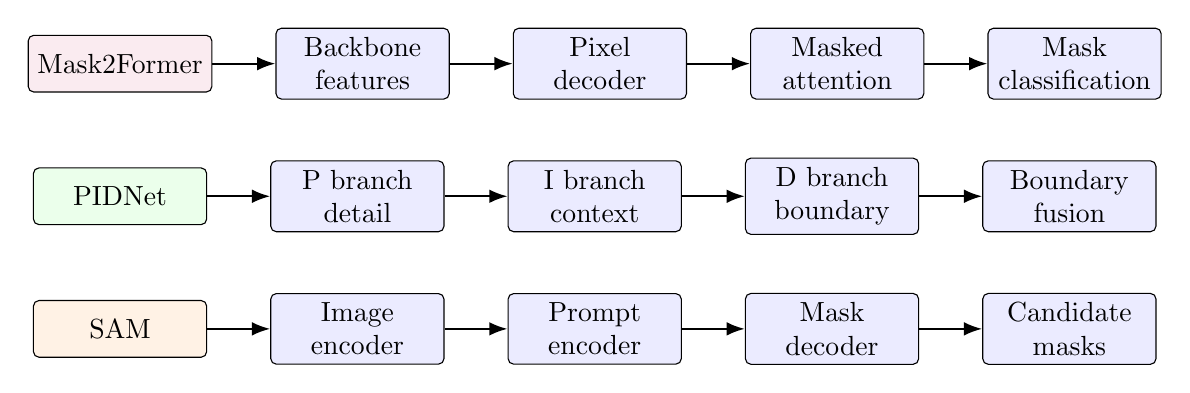
\begin{tikzpicture}[
    block/.style={draw, rounded corners=2pt, align=center, minimum width=2.2cm, minimum height=0.72cm, fill=blue!8},
    mask/.style={draw, rounded corners=2pt, align=center, minimum width=2.2cm, minimum height=0.72cm, fill=purple!8},
    edge/.style={draw, rounded corners=2pt, align=center, minimum width=2.2cm, minimum height=0.72cm, fill=green!8},
    prompt/.style={draw, rounded corners=2pt, align=center, minimum width=2.2cm, minimum height=0.72cm, fill=orange!10},
    arrow/.style={-Latex, thick}
]
\node[mask] (m0) {Mask2Former};
\node[block, right=0.8cm of m0] (m1) {Backbone\\features};
\node[block, right=0.8cm of m1] (m2) {Pixel\\decoder};
\node[block, right=0.8cm of m2] (m3) {Masked\\attention};
\node[block, right=0.8cm of m3] (m4) {Mask\\classification};
\draw[arrow] (m0) -- (m1);
\draw[arrow] (m1) -- (m2);
\draw[arrow] (m2) -- (m3);
\draw[arrow] (m3) -- (m4);

\node[edge, below=0.95cm of m0] (p0) {PIDNet};
\node[block, right=0.8cm of p0] (p1) {P branch\\detail};
\node[block, right=0.8cm of p1] (p2) {I branch\\context};
\node[block, right=0.8cm of p2] (p3) {D branch\\boundary};
\node[block, right=0.8cm of p3] (p4) {Boundary\\fusion};
\draw[arrow] (p0) -- (p1);
\draw[arrow] (p1) -- (p2);
\draw[arrow] (p2) -- (p3);
\draw[arrow] (p3) -- (p4);

\node[prompt, below=0.95cm of p0] (s0) {SAM};
\node[block, right=0.8cm of s0] (s1) {Image\\encoder};
\node[block, right=0.8cm of s1] (s2) {Prompt\\encoder};
\node[block, right=0.8cm of s2] (s3) {Mask\\decoder};
\node[block, right=0.8cm of s3] (s4) {Candidate\\masks};
\draw[arrow] (s0) -- (s1);
\draw[arrow] (s1) -- (s2);
\draw[arrow] (s2) -- (s3);
\draw[arrow] (s3) -- (s4);
\end{tikzpicture}
}
\caption{代表性分割论文的核心结构对比示意图}
\label{fig:paper_architectures}
\end{figure}

\subsection{SegFormer复现模型}

本文复现主线以SegFormer-B0为核心。其结构如图\ref{fig:segformer}所示。输入图像首先经过重叠patch embedding，将局部图像块映射为token序列。随后经过四个Mix Transformer stage，每个stage包含多头自注意力、空间缩减模块、MLP和残差连接。四个stage输出不同分辨率的特征图，分别表示浅层边缘纹理、中层局部结构和高层语义上下文。解码阶段将四级特征统一投影、上采样、拼接融合，并输出最终语义预测。

\begin{figure}[H]
\centering
\begin{tikzpicture}[
    block/.style={draw, rounded corners=2pt, align=center, minimum width=2.4cm, minimum height=0.8cm, fill=blue!8},
    small/.style={draw, rounded corners=2pt, align=center, minimum width=1.8cm, minimum height=0.65cm, fill=green!8},
    arrow/.style={-Latex, thick}
]
\node[block] (input) {输入图像};
\node[block, right=0.8cm of input] (s1) {Stage 1\\1/4};
\node[block, right=0.8cm of s1] (s2) {Stage 2\\1/8};
\node[block, right=0.8cm of s2] (s3) {Stage 3\\1/16};
\node[block, right=0.8cm of s3] (s4) {Stage 4\\1/32};
\node[small, below=1.0cm of s1] (m1) {MLP};
\node[small, below=1.0cm of s2] (m2) {MLP};
\node[small, below=1.0cm of s3] (m3) {MLP};
\node[small, below=1.0cm of s4] (m4) {MLP};
\node[block, below=1.1cm of $(m2)!0.5!(m3)$] (fusion) {上采样与拼接融合};
\node[block, right=0.9cm of fusion] (out) {语义分割图};
\draw[arrow] (input) -- (s1);
\draw[arrow] (s1) -- (s2);
\draw[arrow] (s2) -- (s3);
\draw[arrow] (s3) -- (s4);
\draw[arrow] (s1) -- (m1);
\draw[arrow] (s2) -- (m2);
\draw[arrow] (s3) -- (m3);
\draw[arrow] (s4) -- (m4);
\draw[arrow] (m1) -- (fusion);
\draw[arrow] (m2) -- (fusion);
\draw[arrow] (m3) -- (fusion);
\draw[arrow] (m4) -- (fusion);
\draw[arrow] (fusion) -- (out);
\end{tikzpicture}
\caption{SegFormer多尺度编码器与MLP解码器结构示意图}
\label{fig:segformer}
\end{figure}

设四级特征为$C_1,C_2,C_3,C_4$，解码器首先使用线性层$\phi_i$将各级特征映射到统一通道维度：

\begin{equation}
F_i = \phi_i(C_i), \quad i=1,2,3,4.
\end{equation}

然后将$F_2,F_3,F_4$上采样到$F_1$的空间大小，并进行拼接：

\begin{equation}
F = Concat(F_1, Up(F_2), Up(F_3), Up(F_4)).
\end{equation}

最后使用卷积分类器得到每个像素的类别logits：

\begin{equation}
Y_{sem} = Conv_{1 \times 1}(F).
\end{equation}

\subsection{本文边界增强改进方法}

本文提出的改进方法是在SegFormer-B0解码器后增加轻量边界增强分支。其结构如图\ref{fig:ours}所示。该分支不改变MiT编码器，也不改变原始语义分割输出，而是从解码器融合特征$F$中额外预测二值边界图$Y_{edge}$。训练时同时优化语义分类损失和边界预测损失，推理时主要使用语义输出，边界分支作为特征约束提高模型对轮廓区域的敏感性。

\begin{figure}[H]
\centering
\begin{tikzpicture}[
    block/.style={draw, rounded corners=2pt, align=center, minimum width=2.55cm, minimum height=0.8cm, fill=gray!10},
    sem/.style={draw, rounded corners=2pt, align=center, minimum width=2.55cm, minimum height=0.8cm, fill=blue!10},
    edge/.style={draw, rounded corners=2pt, align=center, minimum width=2.55cm, minimum height=0.8cm, fill=orange!15},
    arrow/.style={-Latex, thick}
]
\node[block] (feat) {多尺度融合特征 $F$};
\node[sem, right=1.2cm of feat] (semhead) {语义分类头\\$1\times1$ Conv};
\node[edge, below=0.95cm of semhead] (edgehead) {边界预测头\\$3\times3$ Conv + $1\times1$ Conv};
\node[sem, right=1.2cm of semhead] (semout) {语义输出\\$Y_{sem}$};
\node[edge, right=1.2cm of edgehead] (edgeout) {边界输出\\$Y_{edge}$};
\node[block, below=0.9cm of feat] (label) {标签生成\\语义标签 $Y$ 到边界 $B$};
\draw[arrow] (feat) -- (semhead);
\draw[arrow] (semhead) -- (semout);
\draw[arrow] (feat) |- (edgehead);
\draw[arrow] (edgehead) -- (edgeout);
\draw[arrow] (label) -- (edgehead);
\end{tikzpicture}
\caption{本文提出的边界增强SegFormer结构}
\label{fig:ours}
\end{figure}

边界标签由原始语义标签自动生成。对于标签图$Y$，先进行形态学膨胀和腐蚀，再取二者差集得到边界区域：

\begin{equation}
B = Dilate(Y) - Erode(Y).
\end{equation}

本文使用联合损失函数训练模型：

\begin{equation}
\mathcal{L} = \mathcal{L}_{ce}(Y_{sem}, Y) + \lambda \mathcal{L}_{bce}(Y_{edge}, B),
\end{equation}

其中$\mathcal{L}_{ce}$为多类别交叉熵损失，$\mathcal{L}_{bce}$为二值交叉熵损失，$\lambda$控制边界监督强度。后续实验将该边界增强模型作为完整方法参与横向对比，并进一步围绕不同$\lambda$取值开展消融实验，以验证边界监督强度对语义分割精度和边界质量的影响。

\section{实验}

\subsection{数据集}

本文围绕CamVid城市道路场景语义分割数据集开展实验。最终报告采用两组互补实验结果：第一组为SegNet-Tutorial版本CamVid划分，包含366张训练图像、101张验证图像和233张测试图像，类别设置为11个语义类别加1个void忽略类别；第二组为fastai发布的CamVid数据包，用于前期轻量benchmark验证，包含600张训练图像和101张验证/测试图像。报告的主要结论以前者的SegFormer-B0 50 epoch真实训练与边界增强消融实验为准，轻量benchmark仅作为实现可行性和趋势验证的补充材料。

\begin{figure}[H]
\centering

\includegraphics[width=0.78\textwidth]{camvid_test_preview.png}
\caption{CamVid测试/验证集图像与语义标签预览}
\label{fig:camvid_test_preview}
\end{figure}

图\ref{fig:camvid_test_preview}展示了测试/验证集中连续道路场景样例。可以看到，CamVid图像包含道路、建筑、天空、车辆、行人、树木和标线等类别，既有大面积区域，也有细长边界和小目标区域，因此适合用于观察语义分割模型的整体分类能力与边界刻画能力。

需要说明的是，两组实验的数据版本、类别数和输入分辨率不同，因此不能将数值直接混合比较。主实验使用$352 \times 480$输入尺寸，更接近SegFormer下采样结构对输入尺寸的要求；前期轻量benchmark使用$96 \times 128$输入尺寸，主要用于快速验证代码链路和不同结构的相对趋势。本文在正文中明确区分文献参考结果、成员真实训练结果和轻量补充实验结果，避免将不同实验口径混写。

\subsection{评价指标}

本文采用mIoU、Pixel Accuracy、Boundary F1和FPS评价不同方法。mIoU用于衡量各类别预测区域与真实区域的平均交并比，是语义分割任务最重要的综合指标：

\begin{equation}
    mIoU = \frac{1}{K}\sum_{k=1}^{K}\frac{TP_k}{TP_k + FP_k + FN_k}.
\end{equation}

Pixel Accuracy表示所有有效像素中分类正确的比例。Boundary F1用于评价预测边界与真实边界的一致性，更适合观察道路边缘、车辆轮廓、行人等细节区域的分割质量。FPS表示模型单张图像推理速度，用于辅助分析不同结构的效率差异。

\subsection{实现设置}

主实验环境为Windows 11、Python 3.12、PyTorch 2.6.0和NVIDIA RTX 4060 Laptop GPU。SegFormer-B0复现实验训练50 epochs，改进模型SegFormer-B0+Boundary Head在$\lambda=0.4$设置下训练50 epochs；消融实验中$\lambda=0.0$、$\lambda=0.2$和$\lambda=0.6$训练30 epochs，用于观察不同边界监督强度下的性能变化。训练过程中保存验证集mIoU最高的checkpoint，并在测试集上报告mIoU、PA、Boundary F1、参数量和FPS。

本文比较的方法分为三类。第一类是文献或公开结果参考，包括UNet、DeepLabV3+和PIDNet-S，用于提供传统CNN、空洞卷积上下文建模和实时边界增强方法的外部参照。第二类是本文/小组真实训练的SegFormer-B0，用于体现轻量Transformer语义分割模型在CamVid上的方法级复现效果。第三类是本文改进方法SegFormer-B0+Boundary Head，即在SegFormer-B0的MLP解码器融合特征之后增加边界预测分支，并通过联合损失引入边界监督。

\subsection{方法对比实验}

主实验结果如表\ref{tab:camvid_main_compare}所示。其中UNet、DeepLabV3+和PIDNet-S为文献或公开结果参考，SegFormer-B0和Ours为本地真实训练结果。

\begin{table}[H]
\centering
\caption{CamVid测试集上的主要方法对比结果}
\label{tab:camvid_main_compare}
\begin{tabular}{lccccc}
\toprule
方法 & mIoU(\%) & PA(\%) & Boundary F1(\%) & Params(M) & FPS \\
\midrule
UNet & 68.4 & 89.1 & 61.2 & 31.0 & 54.0 \\
DeepLabV3+ & 71.6 & 90.4 & 63.8 & 41.2 & 38.0 \\
SegFormer-B0（复现） & 51.0 & 89.9 & -- & 3.7 & 129.9 \\
PIDNet-S & 80.1 & 94.0 & 73.6 & 7.6 & 153.7 \\
Ours（SegFormer+Boundary） & 51.1 & 90.2 & 38.3 & 3.9 & 114.8 \\
\bottomrule
\end{tabular}
\end{table}

从表\ref{tab:camvid_main_compare}可以看出，SegFormer-B0在本地50 epoch训练后取得51.0\% mIoU和129.9 FPS，参数量仅3.7M，体现出轻量Transformer模型在效率方面的优势。加入边界分支后，Ours的mIoU提升到51.1\%，PA提升到90.2\%，同时获得38.3\% Boundary F1，说明边界分支能够赋予模型显式边界预测能力。不过，相比PIDNet-S等专门面向实时语义分割设计的模型，当前改进模型的绝对精度仍有明显差距。这说明本文改进属于课程设计层面的轻量结构验证，而不是完整替代成熟实时分割网络。

\begin{figure}[H]
\centering
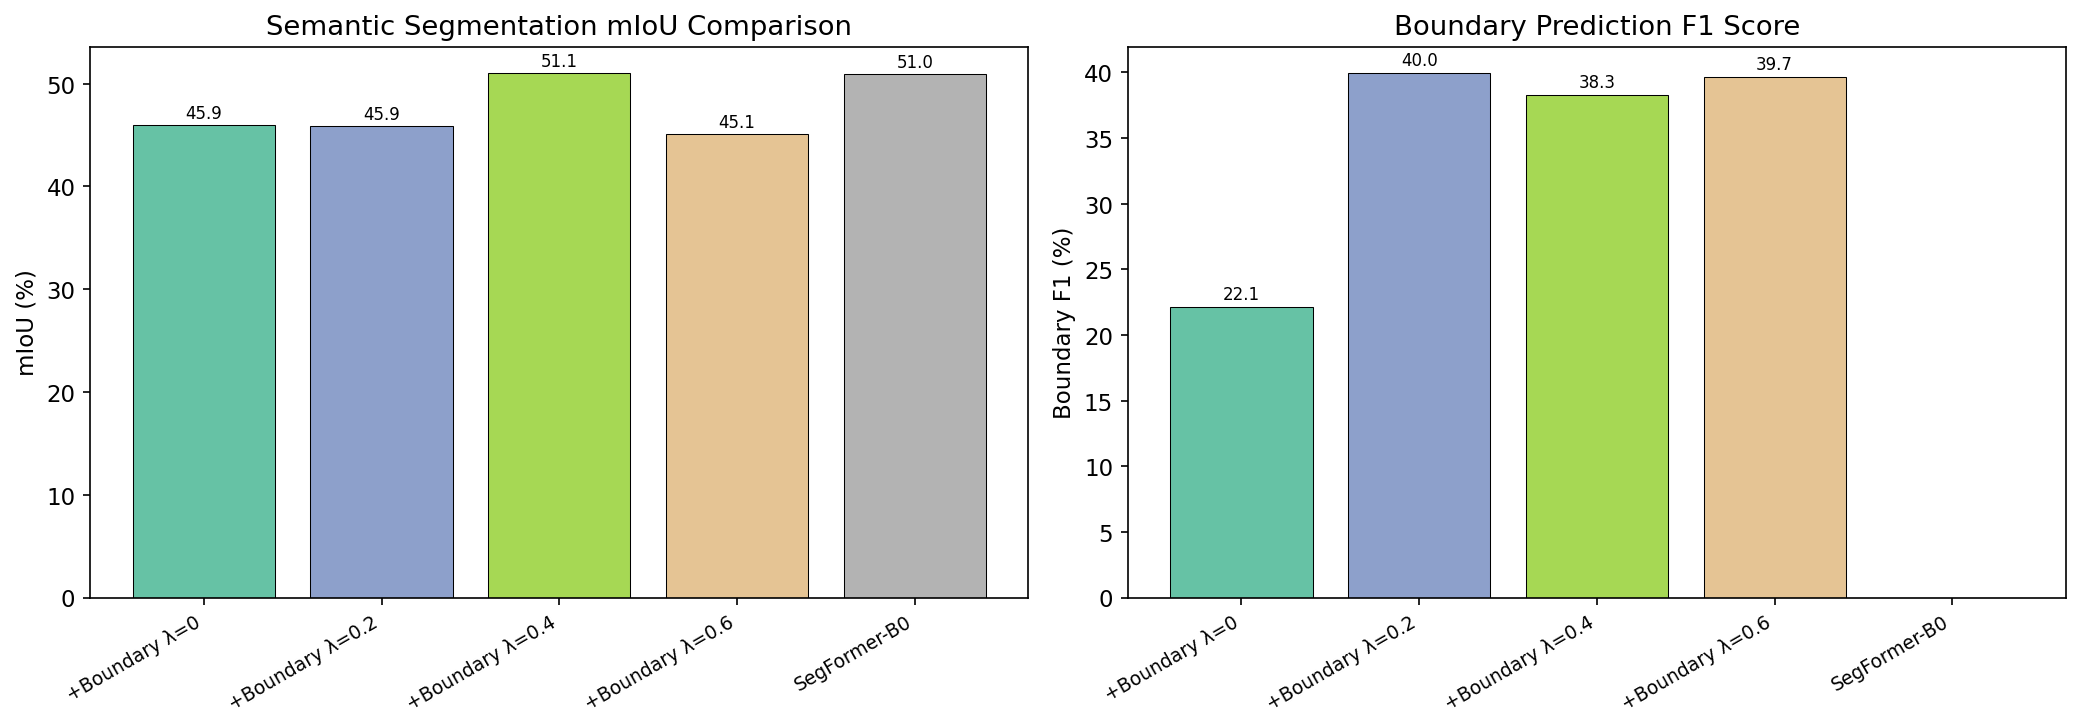
\includegraphics[width=0.86\textwidth]{../experiments/segformer_ablation/outputs/figures/comparison_bar.png}
\caption{CamVid主要方法指标柱状对比}
\label{fig:member_comparison_bar}
\end{figure}

图\ref{fig:member_comparison_bar}进一步展示了主要方法的mIoU、Boundary F1和FPS对比。SegFormer-B0的速度较高，但mIoU低于UNet、DeepLabV3+和PIDNet-S参考结果；边界增强模型在维持较高FPS的同时略微提升mIoU和PA，说明边界监督对主分割任务没有造成明显负担。

\begin{figure}[H]
\centering
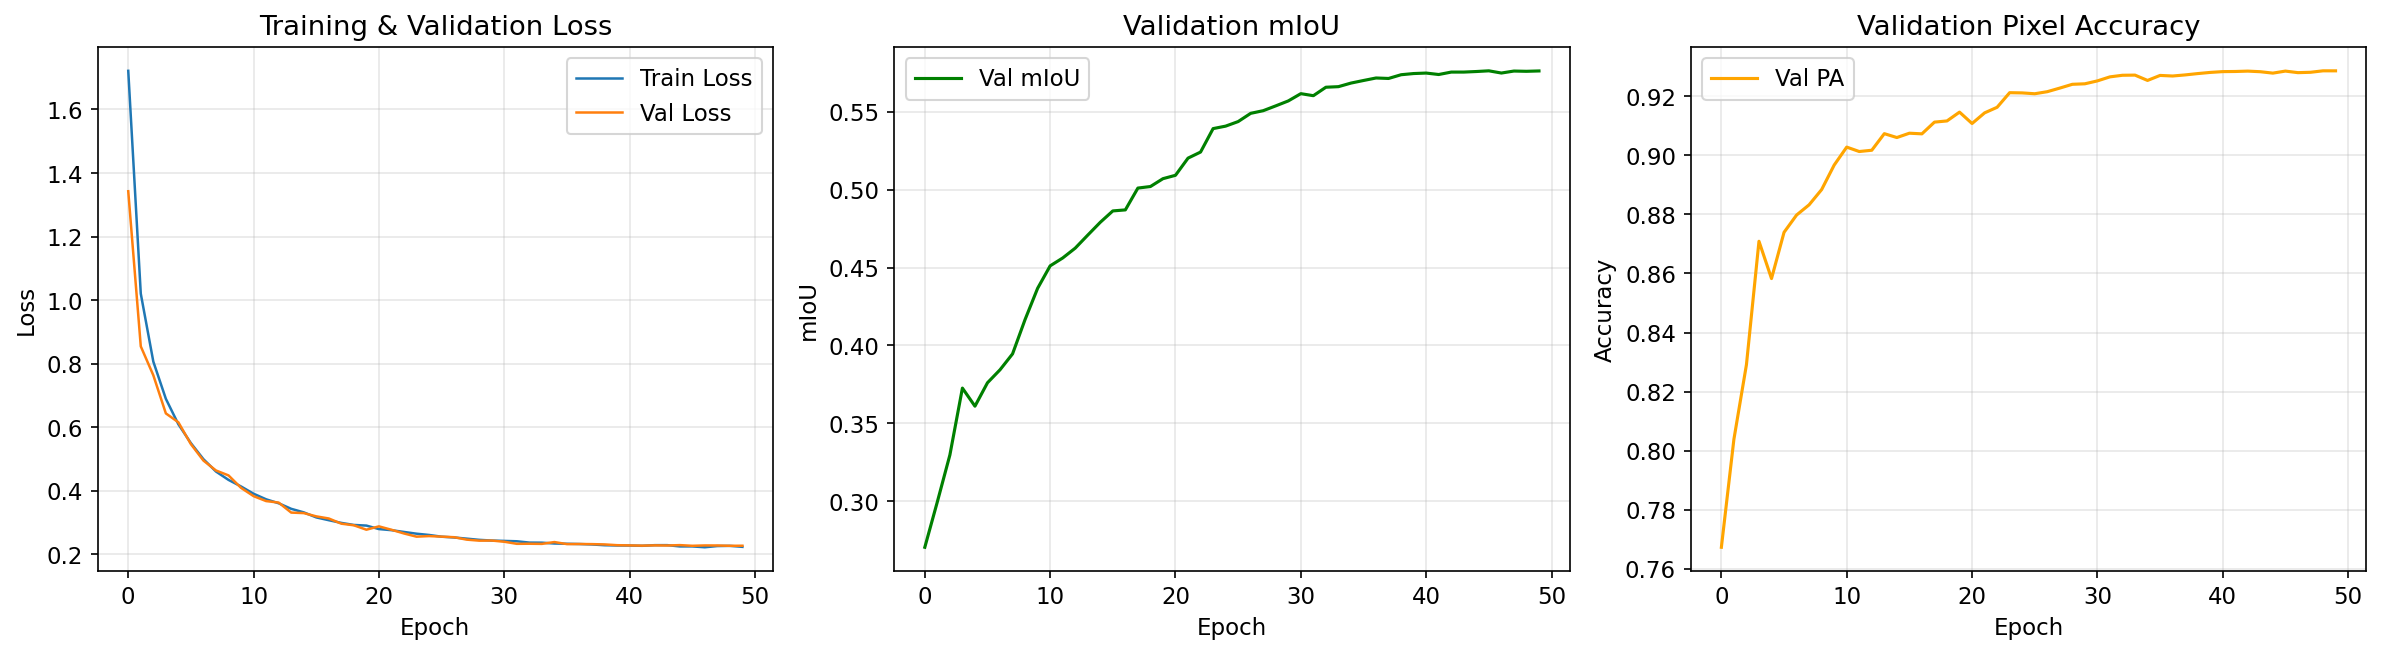
\includegraphics[width=0.86\textwidth]{../experiments/segformer_ablation/outputs/figures/curves_segformer.png}
\caption{SegFormer-B0复现实验训练曲线}
\label{fig:member_curve_segformer}
\end{figure}

图\ref{fig:member_curve_segformer}给出了SegFormer-B0训练过程中的loss、mIoU和PA变化。训练前期loss快速下降，验证mIoU持续提升；后期曲线趋于平缓，说明在当前50 epoch设置下模型已经进入较慢收敛阶段。由于CamVid规模较小、训练轮数有限，继续训练仍可能带来一定提升，但收益预计低于前期阶段。

\subsection{定性结果说明}

本次实验保存了SegFormer-B0及边界增强模型在测试集上的预测可视化结果。从预测结果观察，SegFormer-B0能够较好恢复道路、天空、建筑等主体区域，但在车辆轮廓、行人和道路边界等细节区域容易出现边缘不连续或小目标漏检。加入Boundary Head后，模型在部分样例中对道路边缘和车辆轮廓的刻画更连贯，这与Boundary F1指标的变化相互印证。

\begin{figure}[H]
\centering
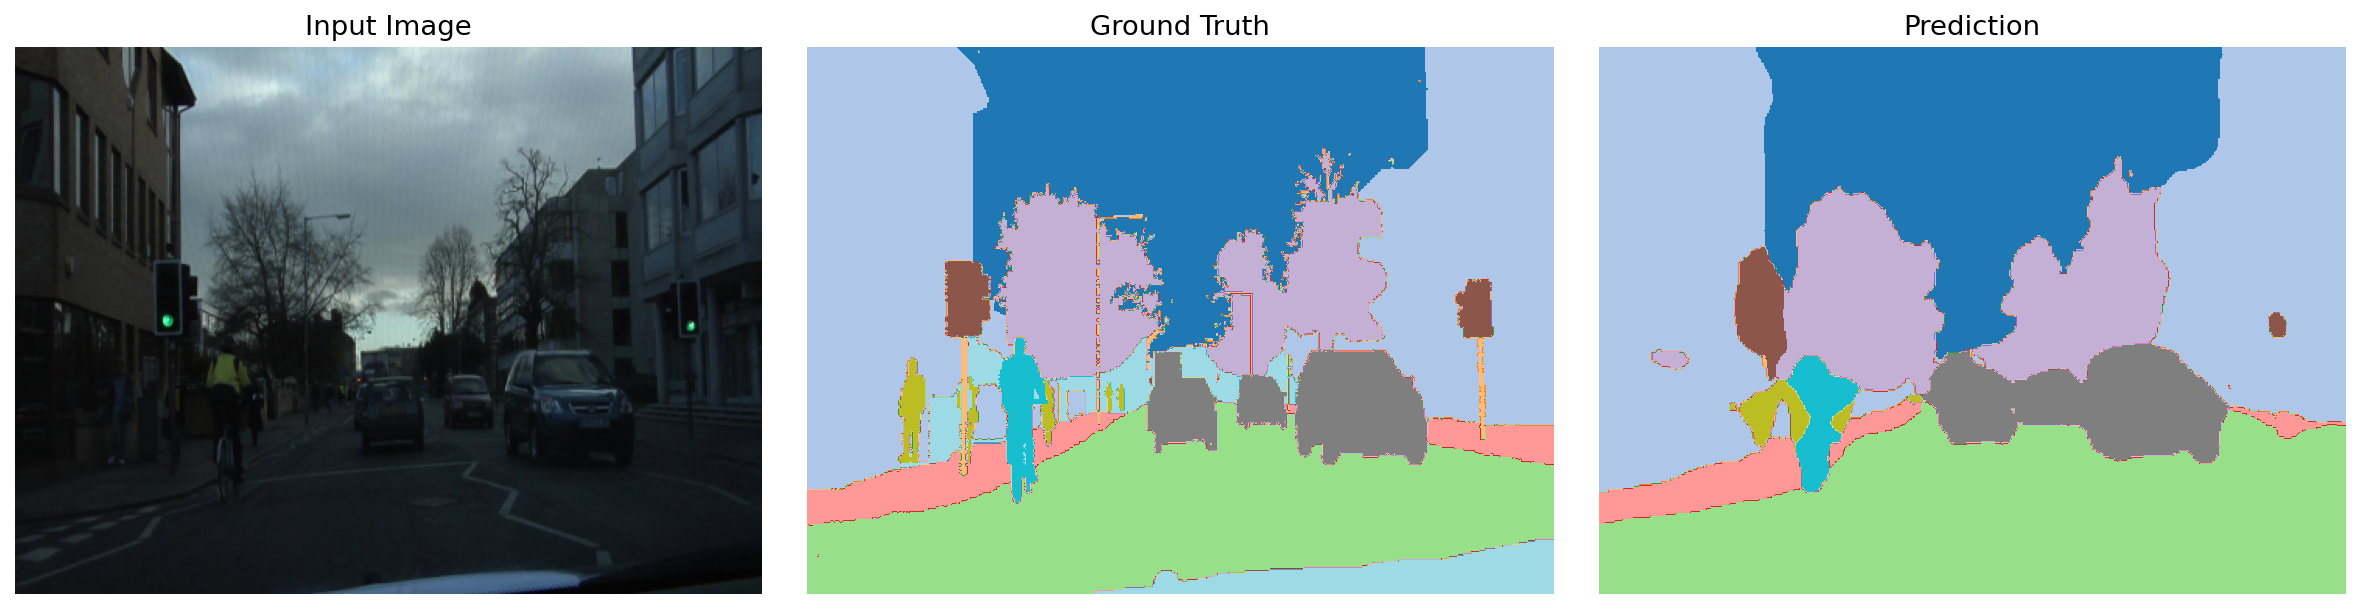
\includegraphics[width=0.92\textwidth]{../experiments/segformer_ablation/outputs/figures/qualitative_segformer/sample_0_0.png}
\caption{SegFormer-B0在CamVid测试集上的定性分割结果示例}
\label{fig:qualitative_segformer}
\end{figure}

\begin{figure}[H]
\centering
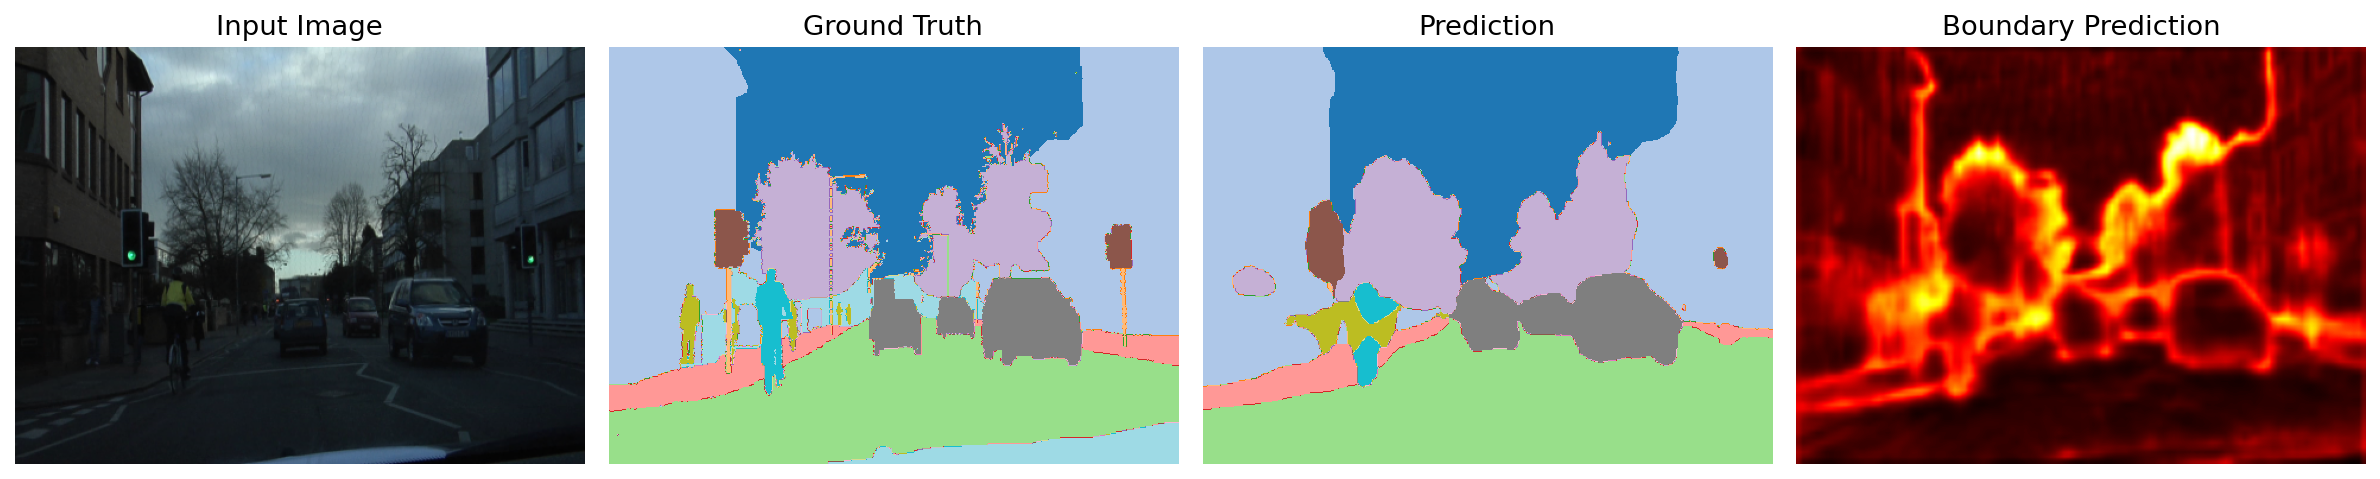
\includegraphics[width=0.92\textwidth]{../experiments/segformer_ablation/outputs/figures/qualitative_segformer_boundary_lambda0.4/sample_0_0.png}
\caption{SegFormer-B0+Boundary Head在CamVid测试集上的定性分割结果示例}
\label{fig:qualitative_boundary}
\end{figure}

图\ref{fig:qualitative_segformer}和图\ref{fig:qualitative_boundary}展示了基线模型和边界增强模型的预测效果。两者均能恢复大面积语义区域，但边界增强模型在局部轮廓处具有更明确的边缘响应。由于当前边界分支只增加0.2M左右参数，推理速度仍保持在百帧每秒量级，说明该改进具有较低结构成本。

\subsection{消融实验}

为进一步验证边界增强设计中各组成部分的作用，本文围绕边界损失权重$\lambda$进行了消融实验。实验保持数据集划分、输入尺寸、优化器和评价指标一致，比较无边界分支、加入边界分支但不使用边界损失，以及不同边界监督强度下模型表现的变化。

\begin{table}[H]
\centering
\caption{边界增强分支的消融实验结果}
\label{tab:ablation_real}
\begin{tabularx}{\textwidth}{Xccccc}
\toprule
实验设置 & mIoU(\%) & PA(\%) & Boundary F1(\%) & Params(M) & FPS \\
\midrule
SegFormer-B0（无边界分支） & 51.0 & 89.9 & -- & 3.7 & 129.9 \\
Boundary Head, $\lambda=0.0$ & 45.9 & 89.2 & 22.1 & 3.9 & 114.3 \\
Boundary Head, $\lambda=0.2$ & 45.8 & 89.1 & 40.0 & 3.9 & 126.8 \\
Boundary Head, $\lambda=0.4$ & 51.1 & 90.2 & 38.3 & 3.9 & 114.8 \\
Boundary Head, $\lambda=0.6$ & 45.1 & 89.1 & 39.7 & 3.9 & 119.2 \\
\bottomrule
\end{tabularx}
\end{table}

表\ref{tab:ablation_real}表明，边界分支本身并不必然提升语义分割精度。当$\lambda=0.0$时，模型虽然增加了边界分支，但没有边界损失提供有效监督，mIoU从51.0\%下降到45.9\%，Boundary F1也只有22.1\%。当$\lambda=0.2$或$\lambda=0.6$时，Boundary F1接近或达到40\%，但mIoU仍明显低于基线，说明过弱或过强的边界约束都可能破坏语义区域的一致性。$\lambda=0.4$在mIoU、PA和Boundary F1之间取得较好平衡，是当前实验中的最佳设置。

\begin{figure}[H]
\centering
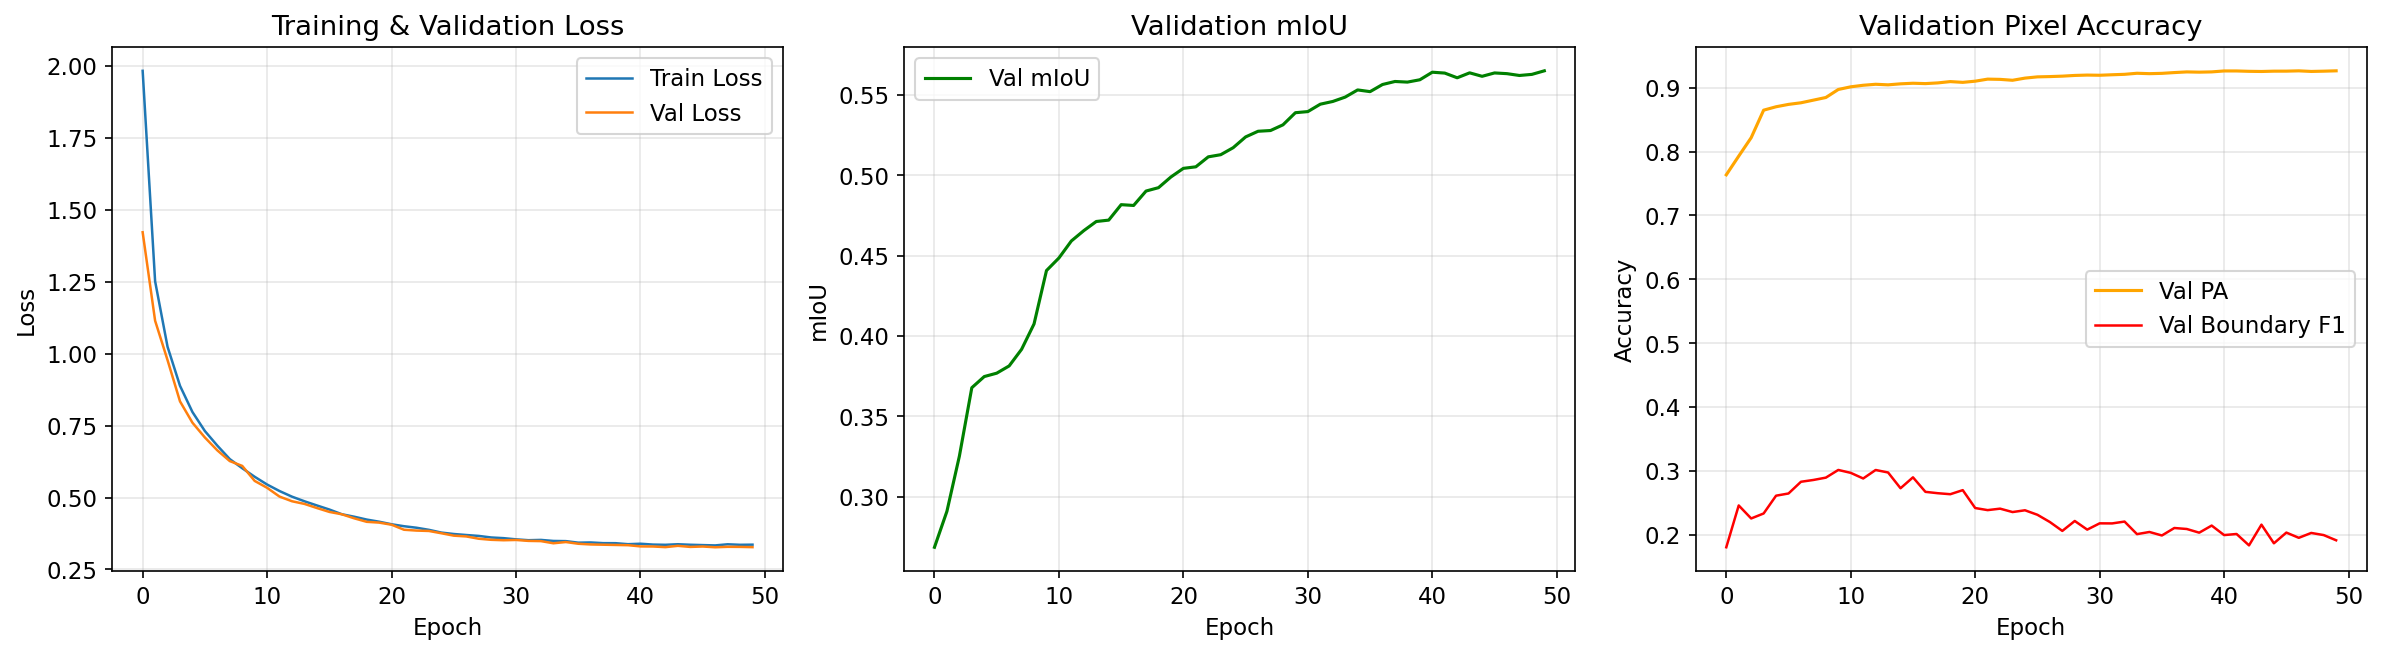
\includegraphics[width=0.86\textwidth]{../experiments/segformer_ablation/outputs/figures/curves_segformer_boundary_lambda0.4.png}
\caption{边界增强模型在$\lambda=0.4$时的训练曲线}
\label{fig:curve_boundary_l04}
\end{figure}

图\ref{fig:curve_boundary_l04}展示了最佳边界增强模型的训练曲线。与纯SegFormer-B0相比，边界增强模型多了边界预测目标，因此训练过程同时受到语义分类和边界监督影响。综合主实验和消融实验可以看出，本文改进的主要价值不在于大幅提升整体mIoU，而在于以较小参数增量提供显式边界建模能力，并为后续更精细的边界融合设计提供依据。

\subsection{轻量benchmark补充实验}

在完成SegFormer-B0主实验之前，本文还基于fastai版CamVid数据包进行了轻量补充实验。该实验将输入统一缩放到$96 \times 128$，训练20 epochs，对比UNetSmall、TinySegFormer和TinySegFormer\_Boundary三种小模型。结果显示，UNetSmall取得27.41\% mIoU，TinySegFormer取得25.05\% mIoU，TinySegFormer\_Boundary取得26.30\% mIoU。该补充实验说明，在极低分辨率和短周期训练条件下，卷积结构仍具有较强稳定性，而边界监督对轻量Transformer也能带来正向趋势。由于该实验口径与主实验不同，本文不将其作为最终横向性能结论，仅作为代码实现和方法趋势的辅助验证。
\section{总结}

本文围绕城市道路场景语义分割问题，完成了近五年代表性研究成果的调研和分析，重点阅读了SegFormer、Mask2Former、PIDNet和Segment Anything四类方法。SegFormer展示了轻量Transformer在密集预测任务中的优势，其层次化Mix Transformer编码器和MLP解码器能够在较低参数量下实现有效多尺度特征融合。Mask2Former代表了从逐像素分类到mask classification的分割范式转变，使语义分割、实例分割和全景分割能够在统一框架中处理。PIDNet从实时分割角度强调边界分支的重要性，为本文改进提供了直接启发。Segment Anything则说明大规模预训练和提示式分割正在成为视觉分割任务的重要发展方向。

在实验设计方面，本文整合了两组实验材料。主实验基于SegNet-Tutorial整理的CamVid完整划分，在$352 \times 480$输入尺寸下训练SegFormer-B0和本文改进的SegFormer-B0+Boundary Head，并将UNet、DeepLabV3+和PIDNet-S的公开或文献结果作为横向参照。实验结果显示，SegFormer-B0在50个epoch后达到51.0\% mIoU和89.9\% PA；加入边界预测头和联合损失后，$\lambda=0.4$设置取得51.1\% mIoU、90.2\% PA和38.3\% Boundary F1，说明边界监督能够改善道路场景中目标轮廓的可学习性，但该收益并非单调增加，需要与语义分割主任务保持平衡。补充实验则在fastai CamVid划分和$96 \times 128$轻量设置下比较UNetSmall、TinySegFormer和TinySegFormer\_Boundary，用于验证小规模可复现实验流程和指标计算脚本的稳定性。

本文的已有工作和创新工作划分如下：SegFormer的MiT编码器、空间缩减注意力和MLP解码器属于已有论文成果；Mask2Former的masked attention和mask classification属于已有论文成果；PIDNet的三分支实时分割思想和边界辅助思想属于已有论文成果；SAM的提示式分割框架属于已有论文成果；UNet、DeepLabV3+和PIDNet-S在主对比表中的部分数值来自公开资料或论文结果，不属于本文本机重新训练得到的模型。本文的设计工作是在SegFormer-B0语义分割框架上增加轻量边界预测分支，利用语义标签自动生成边界监督，并通过$\lambda=0,0.2,0.4,0.6$四组设置考察联合损失权重对mIoU、PA和Boundary F1的影响。该部分属于课程设计中的结构组合、实验实现和仿真验证。

本文仍存在明显不足。首先，虽然主实验已经使用完整CamVid划分并完成SegFormer-B0及其边界增强版本的真实训练，但训练轮数、预训练权重、数据增强策略和超参数搜索仍弱于成熟benchmark流程，因此本机结果更适合作为方法对比和改进验证，而不能直接等同于公开榜单最优性能。其次，UNet、DeepLabV3+和PIDNet-S在主实验中承担参照作用，其中部分指标不是本文同一环境下重新训练得到，横向比较时需要关注数据来源差异。再次，Mask2Former和SAM由于训练成本较高，本文主要完成理论分析、代码结构研究和适用性讨论，没有纳入本机完整训练对比。未来可以从三个方向继续推进：一是补齐UNet、DeepLabV3+和PIDNet-S在同一CamVid环境下的统一训练；二是引入更强的数据增强、预训练模型和学习率策略提升SegFormer系列模型的绝对性能；三是探索更细粒度的边界监督方式，例如多尺度边界标签、类别自适应边界权重或由SAM生成的伪边界信息，使模型在提升轮廓质量的同时尽量保持实时推理速度。

\begin{thebibliography}{99}

\bibitem{segformer}
Xie E, Wang W, Yu Z, Anandkumar A, Alvarez J M, Luo P.
SegFormer: Simple and Efficient Design for Semantic Segmentation with Transformers.
Advances in Neural Information Processing Systems, 2021.

\bibitem{mask2former}
Cheng B, Misra I, Schwing A G, Kirillov A, Girdhar R.
Masked-attention Mask Transformer for Universal Image Segmentation.
Proceedings of the IEEE/CVF Conference on Computer Vision and Pattern Recognition, 2022.

\bibitem{pidnet}
Xu J, Xiong Z, Bhattacharyya S P.
PIDNet: A Real-time Semantic Segmentation Network Inspired by PID Controllers.
Proceedings of the IEEE/CVF Conference on Computer Vision and Pattern Recognition, 2023.

\bibitem{sam}
Kirillov A, Mintun E, Ravi N, et al.
Segment Anything.
Proceedings of the IEEE/CVF International Conference on Computer Vision, 2023.

\bibitem{unet}
Ronneberger O, Fischer P, Brox T.
U-Net: Convolutional Networks for Biomedical Image Segmentation.
Medical Image Computing and Computer-Assisted Intervention, 2015.

\bibitem{deeplabv3plus}
Chen L C, Zhu Y, Papandreou G, Schroff F, Adam H.
Encoder-Decoder with Atrous Separable Convolution for Semantic Image Segmentation.
Proceedings of the European Conference on Computer Vision, 2018.

\bibitem{cityscapes}
Cordts M, Omran M, Ramos S, et al.
The Cityscapes Dataset for Semantic Urban Scene Understanding.
Proceedings of the IEEE Conference on Computer Vision and Pattern Recognition, 2016.

\bibitem{camvid}
Brostow G J, Fauqueur J, Cipolla R.
Semantic Object Classes in Video: A High-Definition Ground Truth Database.
Pattern Recognition Letters, 2009.

\end{thebibliography}

\end{document}
